\include{includes/common_start}
\include{includes/tutBlatt_methods}
\tutnr{1}
\section{Organisatorisches}

\subsection{Organisatorisches}

\begin{frame}
	\frametitle{\texttt{whois tutor}}
	
	\begin{itemize}
		\item \textbf{Michael Vollmer} \\ Michael@trollbu.de \\ Tutorium-Nummer: 20 \\ Mittwoch 15:45, SR -109
	\end{itemize}
\end{frame}

\begin{frame}
	\frametitle{Organisatorisches -- Zum Übungsbetrieb}
	\begin{itemize}
		\item \textbf{Abgabe:} \emph{Handschriftlich} in Gruppen
		\begin{itemize}
			\item Bis zu 3 Personen als Gruppe
			\item Erste Abgabe legt die Gruppe fest
			\item Jede Person muss ein eigenes Blatt abgeben (mit Namen der Gruppenteilnehmer, falls vorhanden)
		\end{itemize}
		\item \textbf{Schein:} 
		\begin{itemize}
			\item Klausurbonus (1 Notenschritt)
			\item (Mindestens) Bei allen bis auf einem Blatt 50\% Punkte
		\end{itemize}
		\item korrigierte Übungsblätter gibt es im Tutorium
		\begin{itemize}
			\item Bei Nichtabholung: Büro 274 Montags 14:00-15:00
		\end{itemize}
	\end{itemize}
\end{frame}
\begin{frame}
	\frametitle{Organisatorisches -- Zum Tutorium}
	\begin{itemize}
	\item Tutoriumsfolien
		\begin{itemize}
			\item \texttt{http://tinyurl.com/tgitutws1314}
		\end{itemize}
		\item E-Mail-Liste geht rum
		\item Stoff soll wiederholt werden
		\item Dabei Fokus auf Übungsbetrieb
		\item Fragen/Vorschläge/Anmerkungen willkommen!
	\end{itemize}
\end{frame}

\section{Endliche Automaten}
\subsection{Deterministische endliche Automaten}
\begin{frame}
\frametitle{Deterministische endliche Automaten}

	\begin{minipage}{0.5 \textwidth}
	 \raggedright{ Ein deterministischer endlicher Automat $M$ ist ein 5-Tupel 
        \[
        M= (Q,\Sigma,\delta,s,F).
        \] }
        \begin{itemize}
        \item $Q$:  endliche Zustandsmenge
        \item $\Sigma$:    endliches Alphabet
        \item $\delta$:   Zustandsübergangsfunktion $Q\times \Sigma \rightarrow Q$
        \item $s$:   Startzustand $\in Q$
        \item $F$:   Endzustandsmenge $\subseteq Q$
        \end{itemize}
	\end{minipage}
	\hfill
    \begin{minipage}{0.45 \textwidth}        
        \begin{center}
        	\includegraphics[scale=1]{images/beispielDEA1.pdf}
        \end{center}
    \end{minipage}
\end{frame}
\subsection{Nichtdeterministische endliche Automaten}
\begin{frame}
\frametitle{Nichtdeterministische endliche Automaten}

	\begin{minipage}{0.5 \textwidth}
        Ein nichtdeterministischer endlicher Automat $M$ ist ein 5-Tupel
        \[
        M= (Q,\Sigma,\delta,s,F).
        \]
        \begin{itemize}
        \item $Q$:  endliche Zustandsmenge
        \item $\Sigma$:    endliches Alphabet
        \item \textcolor{red}{$\delta$:   Zustandsübergangsfunktion $Q\times (\Sigma \cup \varepsilon) \rightarrow \pot(Q)$}
        \item $s$:   Startzustand $\in Q$
        \item $F$:   Endzustandsmenge $\subseteq Q$
        \end{itemize}
\vspace{0.5cm}
	Damit der NEA ein Wort akzeptiert, muss es \emph{einen} akzeptierenden Weg geben.
	
	\end{minipage}
	\hfill
    \begin{minipage}{0.45 \textwidth}        
        \begin{center}
        	\includegraphics[scale=1]{images/beispielNEA.pdf}
        \end{center}
    \end{minipage}
\end{frame}
\begin{frame}
	\frametitle{NEA: Beispiel}
	\begin{figure}
	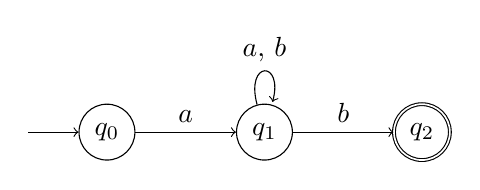
\begin{tikzpicture}
	\node[draw,circle] (q_0) at (0,0) {$q_0$};
	\node[draw,circle] (q_1) at (2,0) {$q_1$};
	\node[draw,circle,double] (q_2) at (4,0) {$q_2$};
	\draw[->] (-1,0) -- (q_0);
	\draw[->] (q_0) -- (q_1) node[midway,anchor=south] {$a$};
	\draw[->] (q_1) -- (q_2) node[midway,anchor=south] {$b$};
	\draw (q_1) edge [loop above] node {$a$, $b$} (q_1);
	\end{tikzpicture}
	\end{figure}
	\begin{itemize}
		\item Eingabe: abb
		\begin{itemize}
			\item $q_0 \xrightarrow{a} q_1 \xrightarrow{b} q_2 \xrightarrow{b} \textcolor{red}{\emptyset}$
			\item $q_0 \xrightarrow{a} q_1 \xrightarrow{b} q_1 \xrightarrow{b} \textcolor{green}{q_2}$
			\item akzeptiert
		\end{itemize}
		\item Eingabe: aba
		\begin{itemize}
			\item $q_0 \xrightarrow{a} q_1 \xrightarrow{b} q_1 \xrightarrow{a} \textcolor{red}{\emptyset}$
			\item $q_0 \xrightarrow{a} q_1 \xrightarrow{b} q_2 \xrightarrow{a} \textcolor{red}{\emptyset}$
			\item akzeptiert nicht
		\end{itemize}
	\end{itemize}
\end{frame}

\section{Reguläre Sprachen}
\subsection{Reguläre Sprachen}
\begin{frame}
\frametitle{Rechtslineare Grammatiken}
Eine Grammatik $G = ( T, V, S, P)$
\begin{itemize}
	\item $T$ = Menge der Terminale (a.k.a. Alphabet der Sprache)
	\item $V$ = Menge der Nichtterminale (zu T disjunkt)
	\item $S \in V$ = Startsymbol
	\item $P \subset V^{+} \times (V \bigcup T)^{*}$ = Menge der Produktionen
\end{itemize}
bei der alle Produktionen so aussehen:
\begin{itemize}
	\item $A \rightarrow \epsilon$
	\begin{itemize}
		\item $A \in V$
		\item $\epsilon$ ist leeres Wort (in der Vorlesung auch $\lambda$)
	\end{itemize}
	\item $A \rightarrow bC$
	\begin{itemize}
		\item $A, C \in V$
		\item $b \in T$
	\end{itemize}
\end{itemize}
heißt rechtslinear bzw. regulär. 
\end{frame}

\begin{frame}
\frametitle{Reguläre Ausdrücke}
$A$ ist ein regulärer Ausdruck über dem Alphabet $\Sigma$ wenn:
\begin{itemize}
	\item $A = \epsilon$
	\item $A = x \in \Sigma$
	\item $A = B^{*} = \{\epsilon, B, BB, BBB, \ldots\}$
	\item $A = B^{+} = \{B, BB, BBB, \ldots\}$
	\item $A = B \cdot C = \{BC\}$
	\item $A = B \mid C = B + C = \{B, C\}$
\end{itemize}
Wobei B und C ebenfalls reguläre Ausdrücke über $\Sigma$ sind.
~\\~\\~\\~\\

Bitte deutlich schreiben:
\begin{equation*}
B^{+}C \neq B + C
\end{equation*}
\end{frame}

\begin{frame}
	\frametitle{Chompsky Typ 3}
	Eine Sprache ist von Chompsky Typ 3, wenn...
	\begin{itemize}
		\item ... sie durch eine reguläre, z.B. rechtslineare, Grammatik angegeben werden kann.
		\item ... sie durch einen regulären Ausdruck angegeben werden kann.
		\item ... ein endlicher Automat angegeben werden kann, der genau diese Sprache akzeptiert.
	\end{itemize}
\end{frame}
\subsection*{Aufgabe 1}
\begin{frame}
	\frametitle{Aufgabe 1}
	\only<1>{
	Gegeben sei der folgende endliche Automat:\\
	$\mathcal{M} = (\mathcal{Q},\Sigma,\delta,S,\mathcal{F})$ mit
	$\Sigma = \{a,b\}$, $\mathcal{Q} = \{S,B,C,D\}$, $\mathcal{F} = \{B,C\}$
	und $\delta$ gegeben durch:
	}
	\only<2>{\vspace{-1.7 cm}}
	\begin{center}
		\resizebox{4cm}{!} {%
		\begin{tikzpicture}[line width=1pt]
			\start{0}{0}{S}
			\totr{0}{0}{1}{1}{a}
			\tobr{0}{0}{1}{-1}{b}
			\final{1}{1}{B}
			\rloopt{1}{1}{a}
			\draw (3,1) node[above right]{$b$};
			\draw [->] (2.283,1.717) -- (3.717,0.283);
			\final{1}{-1}{C}
			\draw (3,-1) node[below right]{$a$};
			\draw [->] (2.283,-1.717) -- (3.717,-0.283);
			\rloopb{1}{-1}{b}
			\state{2}{0}{D}
			\rloopr{2}{0}{a,b}
		\end{tikzpicture}%
		}
	\end{center}
	\only<2>{
	\begin{enumerate}
		\item Geben Sie die von diesem Automaten akzeptierte Sprache in einem regulären
		Ausdruck an!
		\item Um was für einen Automaten handelt es sich?
		\item Konstruieren Sie einen äquivalenten endlichen Automaten, der nur einen
		einzigen Endzustand besitzt!
		\item Geben Sie eine linkslineare Grammatik für die Sprache dieses Automaten an,
		die keine überflüssigen Nichtterminale und Regeln enthält!
	\end{enumerate}
	}
\end{frame}
\subsection{Aufgabe 2}
\begin{frame}
	\frametitle{Aufgabe 2}
	\begin{enumerate}
		\item Formulieren Sie einen regulären Ausdruck über dem Alphabet $\Sigma =
		\{0,1\}$, der jedes beliebige Wort erfasst,\\
		wobei die vorletzte Ziffer $0$ sein soll!
		\item Geben Sie eine rechtslineare Grammatik an.
		\item Geben Sie einen dazugehörigen Automaten an, der diese Sprache akzeptiert!
	\end{enumerate}
\end{frame}

\section{Akzeptor $\leftrightarrow$ Grammatik}
\subsection{Akzeptor $\rightarrow$ Grammatik}
\begin{frame}
	\frametitle{Akzeptor $\rightarrow$ Grammatik}
	Umwandlung von einem endlichen Akzeptor $M = (Q,\Sigma,\delta,q_0,F)$ in eine rechtslineare Grammatik $G = (T,V,S,P)$:
	\begin{enumerate}
		\item $T := \Sigma$.
		\item $\forall q \in Q$ ein Nichtterminalsymbol in $V$ definieren, wobei $S \; q_0$ zugeordnet ist.
		\item $P := \{(X \rightarrow tY) \;\vert\; (q_X,t)=q_Y \in \delta\} \;\bigcup\; \{(Z \rightarrow \lambda) \;\vert\; q_Z \in F\}$.~\\
		Wobei $X$, $Y$ und $Z$ jene Nichtterminalsymbole sind, welche $q_X$, $q_Y$, bzw. $q_Z$ zugeordnet sind. 
	\end{enumerate}
\end{frame}

\subsection{Aufgabe 3}
\begin{frame}
	\frametitle{Aufgabe 3}
	Gegeben sei der folgende endliche Akzeptor $\mathcal{M}$ mit dem Eingabealphabet
	$\Sigma = \{a,b,c,d\}$:
	\begin{center}
		\begin{tikzpicture}[line width=1pt]
			\start{0}{0}{q_0}
			\tor{0}{0}{1}{a,b}
			\state{1}{0}{q_1}
			\rloopt{1}{0}{a,b}
			\totr{1}{0}{3}{1}{c}
			\state{3}{1}{q_2}
			\rloopt{3}{1}{c}
			\draw (8,1) node[above right]{$d$};
			\draw [->] (6.283,1.717) -- (9.717,0.283);
			\final{5}{0}{q_3}
			\tol{5}{0}{1}{d}
		\end{tikzpicture}
	\end{center}
	\begin{enumerate}
		\item Welche Sprache $\mathcal{L}(\mathcal{M})$ wird von dem Akzeptor $\mathcal{M}$
		akzeptiert?
		\item Konstruieren Sie aus $\mathcal{M}$ eine rechtslineare Grammatik, die
		$\mathcal{L}(\mathcal{M})$ erzeugt!
	\end{enumerate}
\end{frame}

\subsection{lineare Grammatik $\rightarrow$ Akzeptor}
\begin{frame}
\frametitle{Konstruktion eines Akzeptors aus einer linearen Grammatik}
Gegeben: rechtslineare Grammatik $G = (T, V, S, P)$~\\
Gesucht: endlicher Akzeptor $M = (Q,\Sigma,\delta,q_0,F)$

\begin{enumerate}
	\item $\Sigma:= T$
	\item $Q:= \{q_X \; \vert \; X \in V\}$
		\begin{itemize}
			\item $q_0 = q_S$
		\end{itemize}
	\item $\delta:= \{ (q_X, t) \rightarrow q_Y \; \vert \; (X \rightarrow tY) \in P \} $	
	\item $F:= \{q_X \; \vert \; (X \rightarrow \lambda) \in P \}$
\end{enumerate}\end{frame}

\subsection{Aufgabe 4}
\begin{frame}
	\frametitle{Aufgabe 4}
	Die Sprache $\mathcal{L}$ sei durch den regulären Ausdruck $(aa^*b^*)^*cc^*$
	definiert.
	\begin{enumerate}
		\item Geben Sie eine rechtslineare Grammatik $\mathcal{G}$ an, die $\mathcal{L}$
		erzeugt!
		\item Konstruieren Sie aus $\mathcal{G}$ einen endlichen Akzeptor, der $\mathcal{L}$
	akzeptiert!
	\end{enumerate}
\end{frame}
\section{Semi-Thue-Systeme}
\subsection{Semi-Thue-Systeme}

\begin{frame}
\frametitle{Semi-Thue-Systeme}
Ein Semi-Thue-System besteht aus
\begin{itemize}
	\item einem nichtleeren Alphabet $A$
\end{itemize}
und
\begin{itemize}
	\item einer Produktionsmenge $P \subset \{A^* \rightarrow A^*\}$
\end{itemize}~\\
Beispiel:~\\
$A = \{a, b, c\}$~\\
$P = \{ab \rightarrow c, bc \rightarrow a, aa \rightarrow \epsilon, cc \rightarrow \epsilon\}$~\\~\\
Beispieleingaben:
\begin{description}
	\item[abc] $\Rightarrow$ cc $\Rightarrow$ $\epsilon$~\\
	$\Rightarrow$ aa $\Rightarrow$ $\epsilon$~\\
	\item[aab] $\Rightarrow$ b~\\
	$\Rightarrow$ ac
\end{description}
Produktionen sind nicht immer eindeutig.
\end{frame}
\begin{frame}
	\frametitle{Scholtens Kaffeedosenspiel}
	Gegeben: 
	\begin{itemize}
		\item Dose mit (endlich vielen) weißen und schwarzen Bohnen (mindestens einer).
		\item Spielregeln: Nehme zufällig 2 Bohnen aus der Dose
		\begin{itemize}
			\item Falls die Bohnen die gleiche Farbe haben, so lege eine schwarze in die Dose zurück.
			\item Falls die Bohnen verschiedene Farben haben, so lege nur die weiße Bohne zurück.
		\end{itemize}
	\end{itemize}
	Behauptungen:
	\begin{enumerate}
		\item Spiel terminiert immer mit genau einer Bohne in der Dose.
		\item Das Ergebnis ist nur von den Farben der Bohnen abhängig.
	\end{enumerate}
\end{frame}
\begin{frame}
	\frametitle{Kaffeebohnen in Semi-Thue}
	Semi-Thue-System:
	\begin{itemize}
		\item A = \{ S, W\}
		\item P = \{ SW $\rightarrow$ W, WS $\rightarrow$ W, SS $\rightarrow$ S,	WW $\rightarrow$ S \}	
	\end{itemize}~\\~\\
	Behauptungen:
	\begin{itemize}
		\item Die Ersetzungen terminieren immer mit Termlänge 1
		\item Das Ergebnis ist unabhängig von der Reihenfolge der Regelanwendungen
	\end{itemize}
\end{frame}

\begin{frame}
	\frametitle{Beweis der Terminierung durch Induktion}
	\begin{itemize}
		\item Induktionsanfang: Term der Länge 1\\
			Keine Regel anwendbar, also terminiert mit Länge 1
		\item Induktionsvoraussetzung: Jeder Term mit einer beliebig aber festen Länge $n$ terminiert mit Länge 1.
		\item Induktionsschritt: Term mit Länge $n + 1$\\
		\begin{itemize}
			\item Da $n$ mindestens 1 ist, besitzt der Term mindestens Länge 2. Also ist auf jeden Fall eine Regel anwendbar
			\item Jede Regel ersetzt einen Subterm der Länge 2 mit einem Term der Länge 1. Nach einer Regelanwendung besitzt der Restterm also nun die Länge $n$.
			\item Nach Induktionsvoraussetzung terminiert dieser Restterm mit Länge 1.
		\end{itemize}
	\end{itemize}
\end{frame}

\begin{frame}
	\frametitle{Beweis der Unabhängigkeit durch Induktion}
	\begin{itemize}
		\item Behauptung: Wenn der Term eine ungerade Anzahl an W enthält, terminiert die Term mit W als letztes Zeichen.
		\item Beweis:
			\begin{itemize}
			\item Induktionsanfang: Term ist Länge 1. Falls der Term eine ungerade Anzahl an W enthält, terminiert der Term mit W.
			\item Induktionsvoraussetzung: Behauptung gilt für alle Terme mit einer beliebig aber festen Länge $n$.
			\item Induktionsschritt: Term mit Länge $n + 1$:
			\begin{itemize}
				\item Die Regeln \{ SW $\rightarrow$ W, WS $\rightarrow$ W, SS $\rightarrow$ S \} erhalten die Anzahl von W im Term.
				\item Die Regel \{ WW $\rightarrow$ S \} veringert die Anzahl von W im Term um 2.
				\item Falls die Anzahl W im Term ungerade war, bleibt dies auch nach Regelanwendung erhalten. Nach Regelanwendung besitzt der Term die Restlänge $n$ und es gilt die Induktionsvoraussetzung.
			\end{itemize}
			\end{itemize}
	\end{itemize}
	Analoger Beweis: Bei gerade Anzahl an W im Term, ist S das letzte Zeichen im Term.
\end{frame}

\section{Schluss}
\subsection{Schluss}

\begin{frame}
\frametitle{Bis zum nächsten Mal!}
\vspace{-0.5cm}
\begin{center}
	\resizebox{11.85cm}{!} {%
	\includegraphics[height=0.8\textheight]{images/xkcd_804.png}%
	}
\end{center}
\end{frame}

\include{includes/common_end}
